\section{DESCRIPCIÓN DE LOS DATOS}

Como se ha comentado anteriormente, la búsqueda por mejorar las condiciones animales en los procesos de crianza ha fomentado la investigación en 
diferentes marcadores biológicos.

El \acrfull{pran}\cite{ObservatorioUPM}, perteneciente a la \acrfull{ETSIAAB}, realiza investigaciones en estas líneas, siendo una principal el bienestar animal en peces, 
usando experimentos como el \textit{NetTest}.

A partir de estas labores anteriores de investigación, se han podido obtener materiales para este trabajo, siendo principalmente videos del experimento junto a sus etiquetas. Para obtener 
estos datos, en sucesivos trabajos del \acrshort{pran} se ha utilizado la herramienta \textit{BORIS}\cite{friardBORISFreeVersatile2016}, que ha permitido anotar diferentes momentos en los que 
ha sucedido un movimiento.

En concreto, el grabado y etiquetado manual se llevó a cabo por los técnicos Juan Enrique Barrios Sánchez\cite{barriossanchezPruebaRedEvaluando2023}  y Almudena Gallego Fernández, bajo la supervisión de los investigadores 
Álvaro De la LLave-Propín y Morris Villarroel Robinson.

Por lo tanto, el etiquetado manual no siempre se ha llevado a cabo por la misma persona, con lo que puede existir un factor de subjetividad que añade error humano a la medición de los 
movimientos de los peces.

\subsection{Conjunto de datos disponibles: videos}

Los videos se pueden separar en 2 subconjuntos dependiendo del momento en el que se realizó la grabación, lo cual se ve reflejado en la calidad de la grabación.

\subsubsection{Videos antiguos}

Para este tipo de videos se cuenta en total de un conjunto de 6 videos completos de un experimento \textit{NetTest} sobre todos los peces de un grupo, pero no se tiene mas información relevante sobre 
los especímenes que aparecen en los videos.

Se tratan de videos en formato \texttt{16:9}, con resolución \texttt{1920x1080}, con la cámara posicionada fija verticalmente encima de una mesa donde se lleva a cabo el experimento. Esto se puede ver 
en la \autoref{fig:ExperimentoAntiguo}. En este caso, el experimento se lleva a cabo con redes negras, lo cual puede ser problemático teniendo en cuenta que los peces tienen 
tonalidades similares al marrón y grises.

\begin{figure}[h]
    \centering
    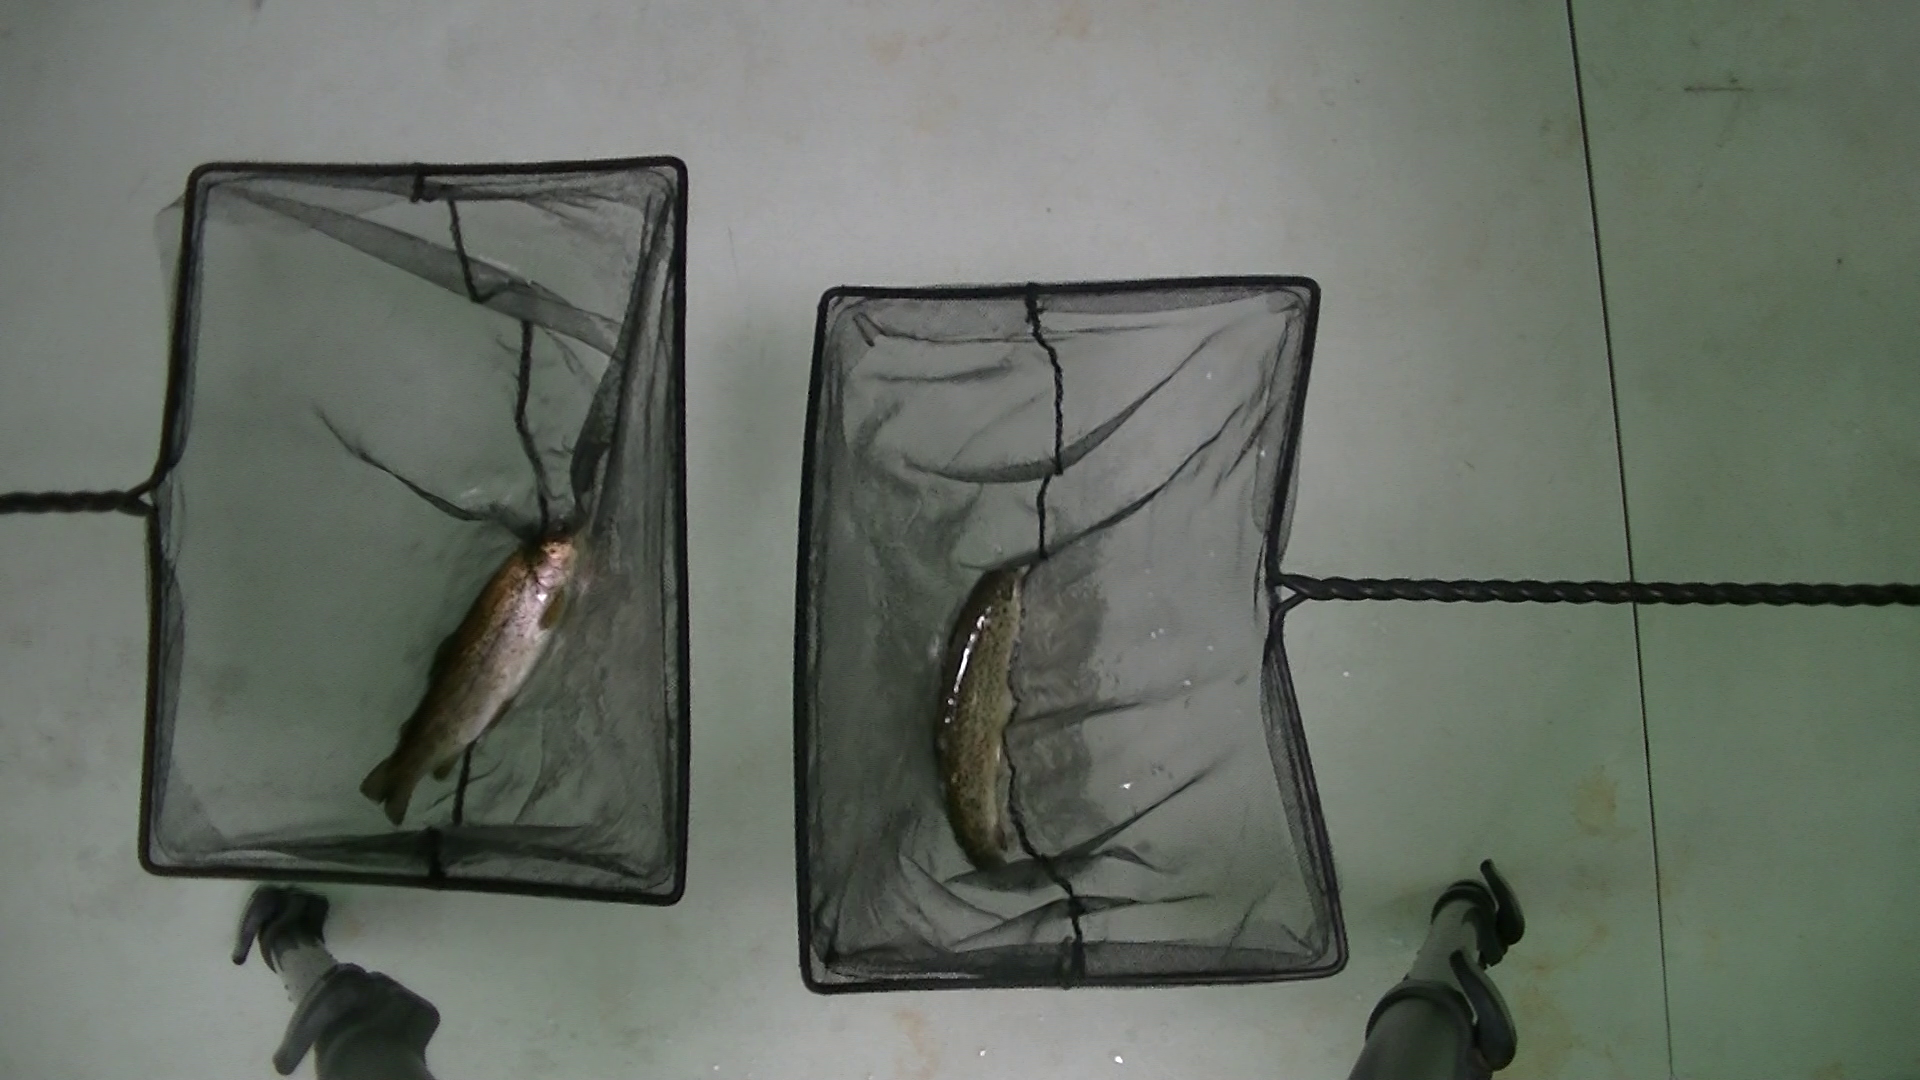
\includegraphics[width=0.70\textwidth]{images/3/ExperimentoAntiguo.png}
    \caption{Aspecto de los videos más antiguos}
    \label{fig:ExperimentoAntiguo}
\end{figure}

Las especificaciones de la cámara en el momento de grabación son desconocidas, pero a través de los detalles de los archivos se observa que son archivos con extensión 
\textit{\acrfull{mts}}, grabados a 25 \acrshort{fps} y con un bitrate (tasa de datos por segundo) de \texttt{16.96 Mbps}.

En estos videos, se realizan el experimento 5 veces con 2 peces a la vez para maximizar el tiempo. Por lo tanto, puede ser necesario segmentarlo manualmente.

Como último punto importante, en estos videos se puede observar que se realiza la variación del \textit{NetTest} que dura 1 minuto aproximadamente.

\subsubsection{Videos nuevos}

Este es el conjunto de datos más amplio y detallado. Cuenta en total con 4 experimentos \textit{NetTest}, en los que se realiza el experimento a 10 jaulas en total (10 peces por jaula). 
Cada jaula consta de un  video que muestra el experimento entero y luego una serie de subvideos que los investigadores de \acrshort{pran} han sacado recortando el original para eliminar 
momentos en los que no hay ningún experimento en pantalla. Esta estructura final se puede ver en la \autoref{fig:EstrucutraNuevos}:

\begin{figure}[h]
    \centering
    \begin{subfigure}[b]{0.5\textwidth}
    \dirtree{%
    .1 \vdots.
    .1 \textbf{Net Test 1}.
    .2 \vdots.
    .1 \textbf{Net Test 2}.
    .2 \vdots.
    .2 \textbf{Jaula 7}.
    .3 \textbf{23 NT R2 J7}.
    .3 \textbf{23 NT R2 J7 P1-2}.
    .3 \vdots.
    .3 \textbf{23 NT R2 J7 P9-10}.
    .2 \vdots.
    .1 \textbf{Net Test 3}.
    .2 \vdots.
    .1 \textbf{Net Test 4}.
    .2 \vdots.
    }
    \end{subfigure}
    \caption{Estructura de los  videos nuevos}
    \label{fig:EstrucutraNuevos}
\end{figure}

Se tiene en cuenta que para los videos siempre se sigue el orden \textit{\acrfull{ltr}}, por lo tanto, para el video \verb|23_NT_R2_J2_P1_2|, el pez de la izquierda será el pez número 1 y 
el pez de la derecha el número 2.

Los videos mantienen las características de formato en \texttt{16:9}, con resolución \texttt{1920x1080} y cámara apuntando verticalmente a la mesa del experimento 
(\autoref{fig:ExperimentoNuevo}), sin embargo, podemos ver que se ha pasado a usar una red verde que aporta cierto contraste respecto al cuerpo del pez. Aparte de esto, 
el marco de la red también ha cambiado y tiene un color plateado.

\begin{figure}[H]
    \centering
    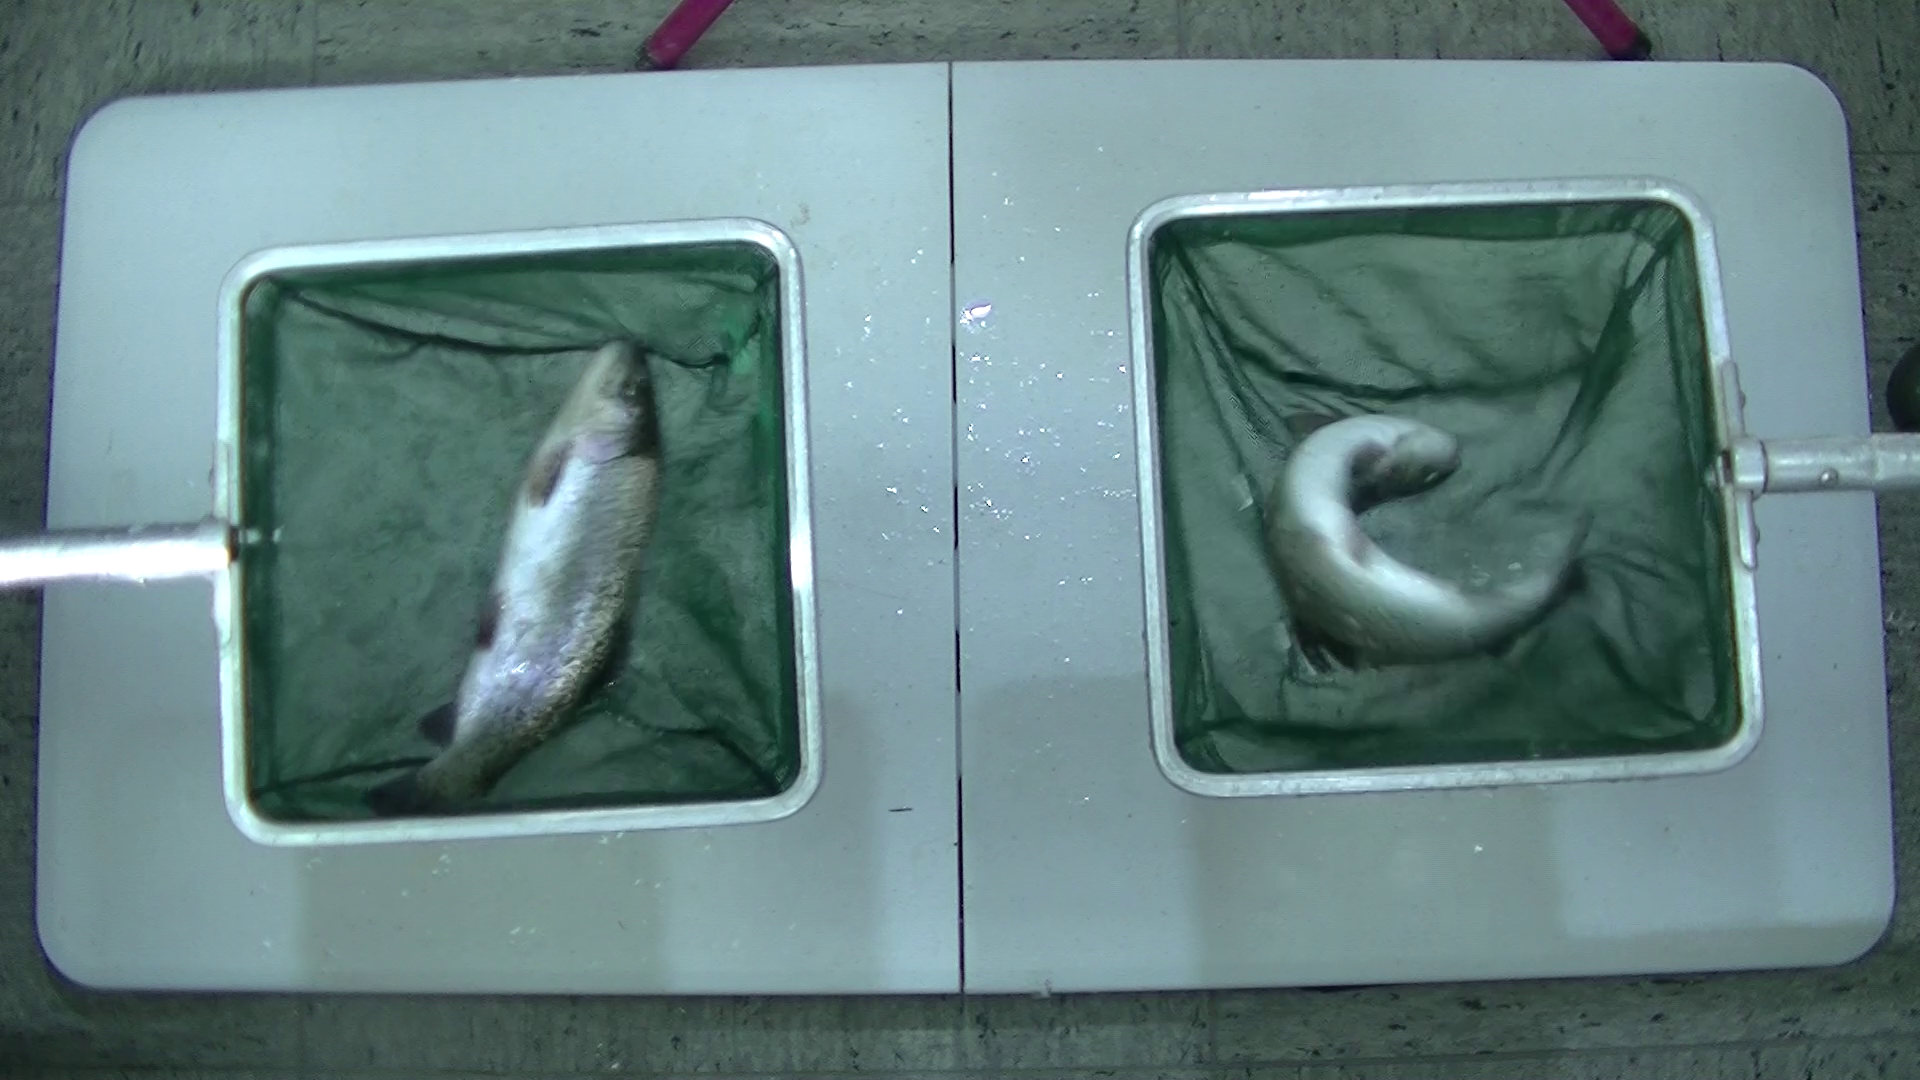
\includegraphics[width=0.7\textwidth]{images/3/ExperimentoNuevo.png}
    \caption{Aspecto de los videos nuevos}
    \label{fig:ExperimentoNuevo}
\end{figure}

Las especificaciones de la cámara para estos videos siguen siendo desconocidas, pero se puede asumir que los parámetros han cambiado por el aumento de la luminosidad de la imagen.
Además, se ha movido un poco la colocación de la mesa y la línea negra queda justo en el medio entre las dos truchas con las que se realiza el experimento.

Respecto a datos técnicos del video, el contenedor ha cambiado a \textit{\acrfull{mov}}, se mantienen los 25 \acrshort{fps} y el bitrate aumenta hasta los \texttt{21 Mbps}.

Los videos obtenidos en este caso también contienen videos de experimentos en grupo, es decir, varios experimentos a varias parejas de truchas. Sin embargo, a diferencia de los videos antiguos, 
en este caso los experimentos \textit{NetTest} duran 15 segundos aproximadamente.

\subsection{Conjunto de datos disponibles: etiquetas}

Por motivos ajenos a este trabajo, no se cuentan con las etiquetas manuales correspondientes a los videos antiguos. Esto implica que no se tiene un marco de referencia para 
contar los movimientos de los videos más antiguos.

\subsubsection{Videos nuevos}

Existen dos archivos Excel, el primero de ellos contiene toda la información sobre los experimentos:
\begin{itemize}
    \item Chip de cada individuo del experimento por grupo, pez y \textit{NetTest}.
    \item Pez de cada grupo y \textit{NetTest}.
    \item Todos los \textit{frames} en los que cada pez ha realizado un movimiento, tomando como referencia el frame 0 del video no recortado.
    \item Momento en el tiempo del video en el que sucede cada movimiento, tomando como referencia el tiempo del video no recortado.
\end{itemize}

De todos los datos, los útiles van a ser los referentes a los movimientos, que se pueden ver en la \autoref{fig:Excel1}.

\begin{figure}[H]
    \centering
    \fbox{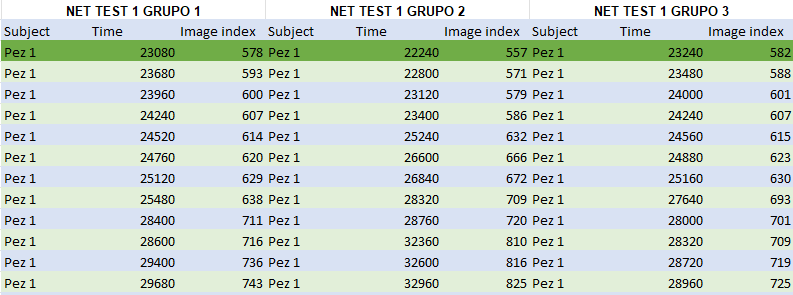
\includegraphics[width=0.7\textwidth]{images/3/Excel1.png}}
    \caption{Columnas del Excel con los datos de \textit{frames} en los que sucede un movimiento}
    \label{fig:Excel1}
\end{figure}
El segundo archivo Excel nos proporciona información ya procesada por los investigadores del \acrshort{pran}, en los cuales aparecen 
los movimientos finales totales para cada pez según grupo y número de experimento \textit{NetTest}. Un ejemplo de una sección del archivo se 
puede ver en la \autoref{fig:Excel2}.

\begin{figure}[H]
    \centering
    \fbox{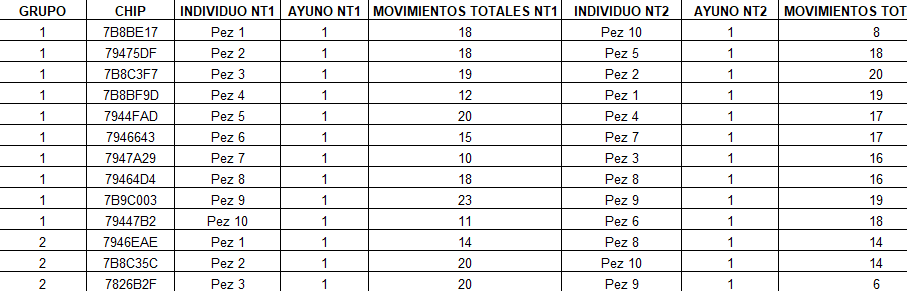
\includegraphics[width=0.7\textwidth]{images/3/Excel2.png}}
    \caption{Sección del archivo de movimientos finales para los videos nuevos}
    \label{fig:Excel2}
\end{figure}

